\chapter{حركية الأقطاب والتحليل الكهربائي}\label{ch:b3:electrode-kinetics}

قطرة دم على شريط بلاستيكي، وخمس ثوانٍ، ثم رقم: جهاز قياس الغلوكوز
الذي يستعمله ملايين الناس مرات عدة في اليوم خلية كهركيميائية،
وما يقيسه ليس فرقًا في الجهد بل تيارًا. يؤكسد إنزيمٌ
الغلوكوز، وينقل معقد ذائب للحديد الإلكترونات إلى قطب من الكربون،
والتيار المار تحدده سرعة انتشار هذا المعقد
نحو القطب، أي تركيزه. ويفسّر هذا الفصل لماذا تعبر
الإلكترونات سطحًا فاصلًا بسرعة أو ببطء (\omterm{thm:b3:electrode-kinetics:butler-volmer}{معادلة بتلر--فولمر})، وكيف
يحدّ انتقال المادة التيار، وكيف تحوّل \omterm{def:b3:electrode-kinetics:cv}{الفولتامترية الدورية} وسائر
طرائق التحليل الكهربائي التيارات إلى تراكيز وثوابت سرعة
وآليات.

\begin{recall}
عرّف مجلد السنة الأولى جهد القطب، والجهد المعياري، 
ومعادلة نرنست، والأقطاب المرجعية وأنصاف الخلايا. وقدّم مجلد السنة الثانية
منحنيات شدة التيار--الجهد بتياراتها المصعدية والمهبطية، 
والقطب العامل والقطب المساعد، وفرط الجهد، والأنظمة السريعة والبطيئة، 
وطبقة الانتشار والتيار الحدي؛ ومعاملات النشاطية والشدة
الأيونية؛ ومنحنيات المعايرة، وطريقة الإضافة القياسية وحد
الكشف. وقدّم \cref{ch:b3:rate-theories} \omterm{def:b3:rate-theories:tst}{نظرية الحالة الانتقالية}. ومن
الفيزياء: قانونا فيك للانتشار، ومعادلة بواسون والمكثفات.
\end{recall}

\begin{omfigure}
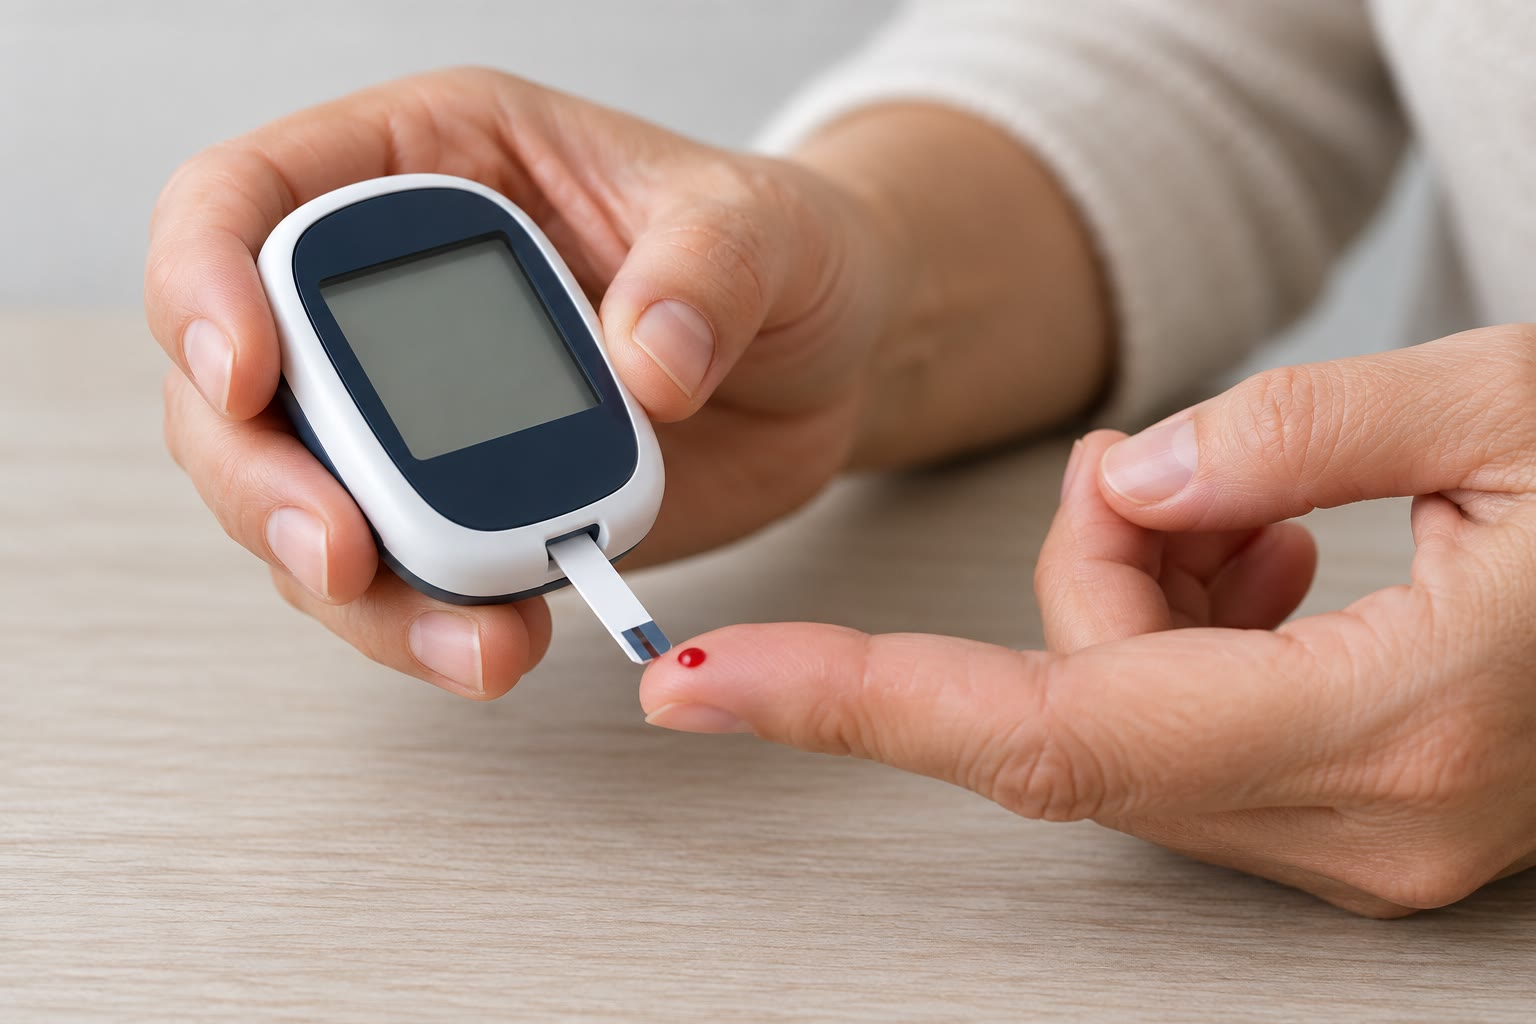
\includegraphics[width=0.6\linewidth]{images/book4/ai/b3-15-glucose-meter.jpg}

{\small جهاز لقياس الغلوكوز في الدم: يحمل الشريط خلية صغيرة جدًا بثلاثة أقطاب
فيها \omterm{def:b3:complex-kinetics:enzyme}{إنزيم} ووسيط أكسدة واختزال؛ ويطبّق الجهاز جهدًا ويقرأ
تيارًا.}
\end{omfigure}

\section{السطح الفاصل بين القطب والمحلول}

يحمل فلزٌّ مغموس في محلول إلكتروليتي شحنةً سطحية، 
ويجيب المحلول بشحنة مساوية لها ومعاكسة، قوامها فائض من أيونات
إشارة واحدة. وتكوّن طبقتا الشحنة مكثفًا سمكه بحجم الجزيئات.

\begin{definition}[الطبقة الكهربائية المزدوجة]\label{def:b3:electrode-kinetics:double-layer}
\emph{الطبقة الكهربائية المزدوجة}\index{طبقة كهربائية مزدوجة} هي
ترتيب الشحنة عند السطح الفاصل بين القطب والمحلول: الشحنة على
الفلز والشحنة الأيونية المعوِّضة في المحلول. وجزؤها المتراص،
\emph{طبقة هلمهولتز}\index{طبقة هلمهولتز}، هو طبقة الأيونات وجزيئات المذيب
الملامسة للسطح؛ و\emph{طبقتها المنتشرة}\index{طبقة منتشرة}
هي المنطقة التي تليها، حيث تنشر الحركة الحرارية الأيونات الفائضة على
مسافة من رتبة \emph{طول ديباي}\index{طول ديباي} $\kappa^{-1}$. 
و\emph{سعة الطبقة المزدوجة}\index{سعة الطبقة المزدوجة} $C_{\mathrm{dl}}$ هي الشحنة
المخزّنة في وحدة المساحة لكل فولت من الجهد عبر السطح الفاصل.
\end{definition}

\begin{proposition}[طول ديباي]\label{prop:b3:electrode-kinetics:debye-length}
في محلول شدته الأيونية $I$ (بوحدة \unit{mol.m^{-3}}) وسماحيته النسبية
$\varepsilon_r$، يتخامد جهد صغير $\varphi_0$ عند القطب داخل المحلول وفق
$\varphi = \varphi_0\eu^{-\kappa x}$، مع
\[
  \kappa^{-1} = \sqrt{\frac{\varepsilon_r\varepsilon_0RT}{2F^2I}} .
\]
\end{proposition}

\begin{proof}
تربط معادلة بواسون (من الفيزياء) الجهد بكثافة الشحنة:
$\dd^2\varphi/\dd x^2 = -\rho/\varepsilon_r\varepsilon_0$. ويخضع كل أيون \omterm{def:b3:partition-functions:boltzmann}{لتوزيع بولتزمان} في
الجهد: $c_i = c_i^{\circ}\eu^{-z_iF\varphi/RT}$، ومنه $\rho = F\sum_iz_ic_i^{\circ}\eu^{-z_iF\varphi/RT}$. ومن أجل $F\varphi \ll RT$،
$\eu^{-z_iF\varphi/RT} \approx 1 - z_iF\varphi/RT$؛ وتتلاشى حدود الرتبة الصفرية بفضل التعادل الكهربائي،
و$\rho \approx -(F^2/RT)\sum_iz_i^2c_i^{\circ}\,\varphi = -(2F^2I/RT)\varphi$. ومنه $\dd^2\varphi/\dd x^2 = \kappa^2\varphi$، 
وحلها الذي ينعدم بعيدًا هو $\varphi_0\eu^{-\kappa x}$.
\end{proof}

\begin{example}[سمك الطبقة المزدوجة]\label{ex:b3:electrode-kinetics:debye}
% ledger: eps:H2O.25C, const:eps0, const:F, const:R
في الماء عند \qty{298.15}{K} ($\varepsilon_r = 78.4$) مع \qty{0.10}{mol/L} من ملح 1:1 ($I = \qty{100}{mol.m^{-3}}$)،
$\kappa^{-1} = \sqrt{78.4 \times \num{8.854e-12} \times 2479/(2 \times 96\,485^2 \times 100)} = \qty{0.96}{nm}$؛ وعند \qty{1.0}{mmol/L}،
أكبر بعشر مرات. \omterm{def:b3:electrode-kinetics:transport}{فالإلكتروليت الداعم} يضغط \omterm{def:b3:electrode-kinetics:double-layer}{الطبقة المنتشرة} إلى بضعة
أقطار جزيئية.
\end{example}

تسلك \omterm{def:b3:electrode-kinetics:double-layer}{الطبقة المنتشرة} سلوك مكثف لوحاه متباعدان بمقدار $\kappa^{-1}$: فسعتها
في وحدة المساحة عند جهد منخفض هي $\varepsilon_r\varepsilon_0\kappa$ (نتيجة غوي--تشابمان؛
ونقبل اعتمادها على الجهد). ومع \omterm{def:b3:electrode-kinetics:double-layer}{طبقة هلمهولتز} المتراصة على التوالي، تعطي
$C_{\mathrm{dl}}$ المقيسة، وهي من رتبة عشرات
الميكروفاراد في السنتيمتر المربع (نموذج شتيرن). وكلما تغير الجهد، يُشحن
هذا المكثف: فالمسح بسرعة $v$ فولت في الثانية يستجرّ تيار شحن $C_{\mathrm{dl}}Av$
لا يحمل أي كيمياء ويضاف إلى كل قياس فولتامتري.

\begin{omfigure}
\begin{tikzpicture}[font=\small, >=Stealth]
  \fill[black!25] (-1.0,0) rectangle (0,3.2);
  \node[rotate=90] at (-0.5,1.6) {\foreignlanguage{arabic}{الفلز}};
  \foreach \y in {0.3,0.8,...,2.9}{\node[font=\scriptsize] at (-0.15,\y) {$-$};}
  \foreach \y in {0.35,0.95,1.55,2.15,2.75}{\draw[omDef, fill=omDef!20] (0.3,\y) circle (0.18); \node[font=\scriptsize] at (0.3,\y) {$+$};}
  \draw[black!50, dashed] (0.55,0) -- (0.55,3.2);
  \node[font=\scriptsize, anchor=south, align=center] at (0.45,3.25) {\foreignlanguage{arabic}{مستوي}\\ \foreignlanguage{arabic}{هلمهولتز}};
  \foreach \x/\y/\s in {1.1/0.6/+, 1.4/2.2/+, 1.9/1.3/+, 2.3/2.7/-, 2.6/0.5/+, 3.1/1.8/+, 3.5/0.9/-, 3.9/2.4/+, 4.4/1.4/-, 4.8/0.4/+, 5.1/2.8/-, 5.4/1.9/+}{
    \draw[black!60, fill=white] (\x,\y) circle (0.15); \node[font=\scriptsize] at (\x,\y) {$\s$};}
  \node[font=\scriptsize, anchor=south] at (3.2,3.25) {\foreignlanguage{arabic}{الطبقة المنتشرة}};
  \draw[->] (0,-2.1) -- (6.0,-2.1) node[anchor=north east] {$x$};
  \draw[->] (0,-2.1) -- (0,-0.3) node[anchor=east] {$|\varphi|$};
  \draw[omThm, thick] (0,-0.5) -- (0.55,-1.0) plot[domain=0.55:5.8, samples=40] (\x,{-2.1+1.1*exp(-(\x-0.55)/1.2)});
  \draw[black!40, dashed] (0.55,-2.1) -- (0.55,-0.4);
  \node[omThm, anchor=south west] at (1.3,-1.6) {$|\varphi(x)|$};
  \draw[<->, black!60] (0.55,-2.5) -- (1.75,-2.5) node[midway, below, font=\scriptsize] {$\sim\kappa^{-1}$};
\end{tikzpicture}

{\small \omterm{def:b3:electrode-kinetics:double-layer}{الطبقة الكهربائية المزدوجة} (نموذج غوي--تشابمان--شتيرن، رسم تخطيطي):
فلز مشحون سالبًا، وطبقة متراصة من الكاتيونات عند مستوي هلمهولتز،
\omterm{def:b3:electrode-kinetics:double-layer}{وطبقة منتشرة} تفوق فيها الكاتيونات الأنيونات عددًا على بضعة أطوال ديباي.
وفي الأسفل، تتناقص قيمة الجهد (السالب، كشحنة الفلز)
خطيًا عبر الطبقة المتراصة، ثم أسيًا في \omterm{def:b3:electrode-kinetics:double-layer}{الطبقة المنتشرة}.}
\end{omfigure}

\section{حركية انتقال الإلكترون}

لنعتبر الاختزال $\mathrm{O} + n\,\mathrm{e}^- \to \mathrm{R}$ على قطب مثبَّت عند الجهد $E$،
وجهد التوازن الموافق للمحلول في كتلته هو $E_{\mathrm{eq}}$. 
وفرط الجهد هو $\eta = E - E_{\mathrm{eq}}$.

\begin{definition}[كثافة تيار التبادل، معامل الانتقال، ثابت السرعة القياسي]\label{def:b3:electrode-kinetics:exchange}
عند التوازن يكون التياران المصعدي والمهبطي متساويين ومتعاكسين؛ 
ومقدارهما المشترك في وحدة المساحة هو \emph{كثافة تيار
التبادل}\index{كثافة تيار التبادل} $j_0$. و\emph{معامل الانتقال}
\index{معامل الانتقال} $\alpha$ ($0 < \alpha < 1$) هو جزء
الطاقة الكهربائية $nF\eta$ الذي يخفض حاجز التفاعل المهبطي. 
و\emph{ثابت السرعة القياسي}\index{ثابت السرعة القياسي} $k^\circ$ هو القيمة
المشتركة لثابتي السرعة المهبطي والمصعدي عند الجهد الشكلي $E^{\circ\prime}$.
\end{definition}

\begin{theorem}[معادلة بتلر--فولمر]\label{thm:b3:electrode-kinetics:butler-volmer}
إذا ساوت التراكيز عند السطح التراكيزَ في كتلة المحلول (دون حدٍّ يفرضه انتقال
المادة)، فإن كثافة التيار عند فرط الجهد $\eta$، مع عدّ التيارات المصعدية
موجبة، هي
\[
  j = j_0\bigl[\eu^{(1 - \alpha)f\eta} - \eu^{-\alpha f\eta}\bigr], \qquad f = \frac{nF}{RT}.
\]
وهذه هي \emph{معادلة بتلر--فولمر}\index{معادلة بتلر--فولمر}.
\end{theorem}

\begin{proof}
بحسب \omterm{def:b3:rate-theories:tst}{نظرية الحالة الانتقالية}، ثابتا السرعة المهبطي والمصعدي هما
$k_{\mathrm c} = A\eu^{-\Delta G_{\mathrm c}^{\ddagger}/RT}$ و$k_{\mathrm a} = A\eu^{-\Delta G_{\mathrm a}^{\ddagger}/RT}$. وتغيير جهد القطب بمقدار $\delta E$
يغيّر طاقة جيبس للتفاعل $\mathrm{O} + n\,\mathrm{e}^- \to \mathrm{R}$ بمقدار $nF\,\delta E$ (فالإلكترونات
في الفلز تكتسب $-nF\,\delta E$ من الطاقة الكهربائية). ولنفترض، في الرتبة الأولى، أن
جزءًا $\alpha$ من هذا التغير يذهب إلى الحاجز المهبطي والباقي إلى
الحاجز المصعدي: $\Delta G_{\mathrm c}^{\ddagger} \to \Delta G_{\mathrm c}^{\ddagger} + \alpha nF\,\delta E$، $\Delta G_{\mathrm a}^{\ddagger} \to \Delta G_{\mathrm a}^{\ddagger} - (1 - \alpha)nF\,\delta E$. وبقياس $\delta E$
انطلاقًا من جهد التوازن، حيث مقدار كل من التيارين $j_0$،
نحصل على $j_{\mathrm c} = j_0\eu^{-\alpha f\eta}$ و$j_{\mathrm a} = j_0\eu^{(1 - \alpha)f\eta}$؛ والتيار الصافي هو
الفرق بينهما.
\end{proof}

\begin{corollary}[مقاومة انتقال الشحنة]\label{cor:b3:electrode-kinetics:linear}
من أجل $|\eta| \ll RT/nF$، $j = j_0f\eta$: فيسلك السطح الفاصل سلوك مقاومة
$R_{\mathrm{ct}} = RT/(nFi_0)$، مع $i_0 = j_0A$.
\end{corollary}

\begin{proof}
ننشر الأسّيين حتى الرتبة الأولى: $j = j_0[(1 - \alpha)f\eta + \alpha f\eta] = j_0f\eta$؛ ثم
$\eta/i = 1/(fi_0)$.
\end{proof}

\begin{corollary}[معادلة تافل]\label{cor:b3:electrode-kinetics:tafel}
من أجل $\eta \ll -RT/nF$ (فرط جهد مهبطي قوي)، يكون الحد المصعدي
مهملًا و
\[
  \eta = \frac{2.303\,RT}{\alpha nF}\bigl(\log j_0 - \log|j|\bigr):
\]
فالمقدار $\log|j|$ خطي في $\eta$، بميل قدره $1/(\text{\qty{118}{mV}})$ لكل عُشر عند \qty{298}{K} من أجل $\alpha = 0.5$، $n =
1$. وهذه هي \emph{معادلة تافل}\index{معادلة تافل}.
\end{corollary}

\begin{proof}
$|j| = j_0\eu^{-\alpha f\eta}$، ومنه $\ln|j| = \ln j_0 - \alpha f\eta$؛ ثم نحوّل إلى اللوغاريتمات العشرية.
\end{proof}

\begin{definition}[مقاومة انتقال الشحنة، ميل تافل]\label{def:b3:electrode-kinetics:charge-transfer}
\emph{مقاومة انتقال الشحنة}\index{مقاومة انتقال الشحنة} لقطب
هي $R_{\mathrm{ct}} = (\partial\eta/\partial i)_{\eta = 0}$. و\emph{ميل تافل}\index{ميل تافل}
هو تغير فرط الجهد لكل عُشر من التيار في منطقة تافل،
$2.303\,RT/\alpha nF$.
\end{definition}

\begin{omfigure}
\begin{tikzpicture}
\begin{axis}[name=bv, omcv, width=0.47\linewidth, height=5.4cm, xmin=-300, xmax=300, ymin=-40, ymax=40,
  xlabel={\babelsublr{$\eta$ / mV}}, ylabel={$j/j_0$},
  legend style={font=\scriptsize, draw=none, at={(0.03,0.97)}, anchor=north west}, legend cell align=left]
\addplot[omDef, thick] table[x=eta_mV, y=a3] {figdata/out/bachelor-3-butler-volmer.dat};
\addplot[black, thick] table[x=eta_mV, y=a5] {figdata/out/bachelor-3-butler-volmer.dat};
\addplot[omThm, thick] table[x=eta_mV, y=a7] {figdata/out/bachelor-3-butler-volmer.dat};
\legend{$\alpha = 0.3$, $\alpha = 0.5$, $\alpha = 0.7$}
\draw[black!30] (axis cs:-300,0) -- (axis cs:300,0) (axis cs:0,-40) -- (axis cs:0,40);
\end{axis}
\begin{axis}[at={(bv.east)}, anchor=west, xshift=1.2cm, omcv, width=0.47\linewidth, height=5.4cm,
  xmin=-300, xmax=300, ymin=-1.5, ymax=4, xlabel={\babelsublr{$\eta$ / mV}}, ylabel={$\log|j/j_0|$},
  unbounded coords=jump]
\addplot[omDef, thick] table[x=eta_mV, y=l3] {figdata/out/bachelor-3-butler-volmer.dat};
\addplot[black, thick] table[x=eta_mV, y=l5] {figdata/out/bachelor-3-butler-volmer.dat};
\addplot[omThm, thick] table[x=eta_mV, y=l7] {figdata/out/bachelor-3-butler-volmer.dat};
\draw[black!40, dashed] (axis cs:-300,2.54) -- (axis cs:0,0);
\draw[black!50] (axis cs:-200,1.85) -- (axis cs:-120,3.3) node[anchor=south, font=\scriptsize, inner sep=1pt] {\foreignlanguage{arabic}{الميل \babelsublr{$1/(\qty{118}{mV})$}}};
\end{axis}
\end{tikzpicture}

{\small \omterm{thm:b3:electrode-kinetics:butler-volmer}{معادلة بتلر--فولمر} ($n = 1$، \qty{298}{K}) لثلاثة معاملات
انتقال. يسارًا: التيار خطي في $\eta$ قرب التوازن (\omterm{def:b3:electrode-kinetics:charge-transfer}{مقاومة
انتقال الشحنة}) وأسّي أبعد من ذلك؛ و$\alpha$ تجعله غير متناظر.
يمينًا: مخطط تافل، الذي يمتد فرعاه المستقيمان إلى $\log|j/j_0| = 0$
عند $\eta = 0$؛ والخط المتقطع هو خط تافل المهبطي من أجل $\alpha = 0.5$.}
\end{omfigure}

\begin{method}[تحليل تافل]\label{met:b3:electrode-kinetics:tafel-analysis}
\begin{enumerate}
  \item سجّل التيار المستقر بدلالة $\eta$ في محلول محرَّك، دون
        التيار الحدي بكثير (أو صحّح أثر انتقال المادة).
  \item ارسم $\log|i|$ بدلالة $\eta$؛ ووفّق الفرع الخطي أبعد من نحو \qty{100}{mV}.
  \item يعطي الميل $\alpha$ (أو $1 - \alpha$ على الفرع المصعدي)؛ ويعطي التقاطع عند $\eta = 0$
        القيمة $\log i_0$.
  \item تحقّق: قرب $\eta = 0$، ميل $i$ بدلالة $\eta$ هو $1/R_{\mathrm{ct}} = nFi_0/RT$.
\end{enumerate}
\end{method}

الأنظمة السريعة والبطيئة في مجلد السنة الثانية هي طرفا هذه
الصورة: فللنظام السريع $j_0$ كبير، ويرتفع منحنى شدة التيار--الجهد عنده
بحدة عند جهد التوازن؛ أما النظام البطيء فيحتاج إلى فرط جهد كبير
قبل أن يمر أي تيار. وتتغير \omterm{def:b3:electrode-kinetics:exchange}{كثافة تيار التبادل} للتفاعل نفسه
على رتب كثيرة من قطب إلى آخر:
فانطلاق الهيدروجين سريع على البلاتين وبطيء جدًا على الزئبق.

\section{انتقال المادة}

\begin{definition}[أنماط انتقال المادة]\label{def:b3:electrode-kinetics:transport}
تبلغ الأنواعُ القطبَ عبر \emph{الهجرة}\index{هجرة}، أي حركة الأيونات
في المجال الكهربائي؛ وبالانتشار، باتجاه تناقص التركيز؛
وعبر \emph{الحمل}\index{حمل}، أي حركة المحلول ككل
(التحريك، والدوران، والجريان). و\emph{الإلكتروليت الداعم}\index{إلكتروليت داعم}
ملح خامل يضاف بفائض كبير، فيحمل كل التيار تقريبًا
عبر المحلول، بحيث لا يتحرك النوع الكهرنشط إلا
بالانتشار والحمل.
\end{definition}

\begin{definition}[قياس التيار الزمني]\label{def:b3:electrode-kinetics:chronoamperometry}
\emph{قياس التيار الزمني}\index{قياس التيار الزمني} يسجّل التيار بدلالة الزمن
بعد قفزة في جهد القطب.
\end{definition}

\begin{theorem}[معادلة كوتريل]\label{thm:b3:electrode-kinetics:cottrell}
بعد قفزة جهد عند $t = 0$ إلى قيمة يُستهلك عندها النوع الكهرنشط
فور بلوغه قطبًا مستويًا مساحته $A$، في محلول ساكن
فيه \omterm{def:b3:electrode-kinetics:transport}{إلكتروليت داعم}، يكون التيار
\[
  i = nFAc^*\sqrt{\frac{D}{\pi t}},
\]
حيث $c^*$ التركيز في كتلة المحلول و$D$ معامل الانتشار. وهذه هي
\emph{معادلة كوتريل}\index{معادلة كوتريل}.
\end{theorem}

\begin{proof}
يخضع التركيز لقانون فيك الثاني $\partial c/\partial t = D\,\partial^2c/\partial x^2$، مع $c(x, 0) = c^*$،
و$c(0, t) = 0$ من أجل $t > 0$ و$c \to c^*$ بعيدًا. والدالة $c = c^*\operatorname{erf}(x/2\sqrt{Dt})$، مع
$\operatorname{erf}u = \frac{2}{\sqrt\pi}\int_0^u\eu^{-s^2}\dd s$، تحقق هذه الشروط: $\operatorname{erf}0 = 0$، $\operatorname{erf}u \to 1$ حين $u \to \infty$
(عند $t \to 0$ لكل $x > 0$، وبعيدًا). ومع $u = x/2\sqrt{Dt}$،
$\partial c/\partial t = c^*\frac{2}{\sqrt\pi}\eu^{-u^2}\partial u/\partial t = -c^*\frac{2}{\sqrt\pi}\eu^{-u^2}\frac{u}{2t}$ و$\partial^2c/\partial x^2 = c^*\frac{2}{\sqrt\pi}(-2u)\eu^{-u^2}\frac{1}{4Dt}$: فيتوافق
طرفا قانون فيك. والتيار هو التدفق عند السطح: $i =
nFAD(\partial c/\partial x)_{x = 0} = nFADc^*\frac{2}{\sqrt\pi}\frac{1}{2\sqrt{Dt}} = nFAc^*\sqrt{D/\pi t}$. (ونقبل وحدانية
الحل.)
\end{proof}

\begin{omfigure}
\begin{tikzpicture}
\begin{axis}[name=pr, width=0.47\linewidth, height=5.2cm, xmin=0, xmax=600, ymin=0, ymax=1.08,
  axis lines=left, xlabel={\babelsublr{$x$ / \unit{\micro m}}}, ylabel={$c/c^*$},
  tick label style={font=\small}, label style={font=\small},
  legend style={font=\scriptsize, draw=none, at={(0.97,0.03)}, anchor=south east}, legend cell align=left]
\addplot[omDef, thick] table[x=x_um, y=t1] {figdata/out/bachelor-3-cottrell-profiles.dat};
\addplot[black!60, thick] table[x=x_um, y=t2] {figdata/out/bachelor-3-cottrell-profiles.dat};
\addplot[omThm, thick] table[x=x_um, y=t3] {figdata/out/bachelor-3-cottrell-profiles.dat};
\addplot[black, thick, dashed] table[x=x_um, y=t4] {figdata/out/bachelor-3-cottrell-profiles.dat};
\legend{\qty{0.1}{s}, \qty{1}{s}, \qty{4}{s}, \qty{16}{s}}
\end{axis}
\begin{axis}[at={(pr.east)}, anchor=west, xshift=1.3cm, width=0.47\linewidth, height=5.2cm,
  xmin=0, xmax=3.3, ymin=0, ymax=40, axis lines=left, xlabel={\babelsublr{$t^{-1/2}$ / \unit{s^{-1/2}}}},
  ylabel={\babelsublr{$i$ / \unit{\micro A}}}, tick label style={font=\small}, label style={font=\small}]
\addplot[omDef, very thick] table[x=tm12, y=i_uA] {figdata/out/bachelor-3-cottrell-current.dat};
\end{axis}
\end{tikzpicture}

{\small \omterm{def:b3:electrode-kinetics:chronoamperometry}{قياس التيار الزمني} (نموذج: $D = \qty{1.0e-5}{cm^2.s^{-1}}$، $c^* = \qty{1.0}{mM}$، قرص قطره \qty{3}{mm}).
يسارًا: تنمو طبقة الاستنزاف وفق $\sqrt{Dt}$، فتبلغ نحو \qty{30}{\micro m} بعد \qty{0.1}{s}
و\qty{350}{\micro m} بعد \qty{16}{s}. يمينًا: تيار كوتريل متناسب مع
$t^{-1/2}$؛ ويعطي ميله $D$.}
\end{omfigure}

يُبقي محلول محرَّك أو قطب قرصي دوّار طبقة الانتشار عند
سمك ثابت $\delta$: فيبلغ التيار القيمة الحدية المستقرة $nFADc^*/\delta$
التي في مجلد السنة الثانية. ومن أجل القرص الدوّار، يتناقص $\delta$ كمقلوب الجذر
التربيعي لسرعة الدوران (ليفيتش، نقبله)، وهذا يجعل التيار الحدي
متناسبًا مع $\sqrt\omega$.

\section{الفولتامترية الدورية}

\begin{definition}[الفولتامترية الدورية]\label{def:b3:electrode-kinetics:cv}
تمسح \emph{الفولتامترية الدورية}\index{فولتامترية دورية} جهد
قطب عامل ساكن خطيًا مع الزمن بين حدّين ذهابًا وإيابًا،
بسرعة مسح $v$، في محلول ساكن، وتسجّل التيار. ومنحنى التيار
بدلالة الجهد هو \emph{الفولتاموغرام}\index{فولتاموغرام}؛ ولكل موجة
\emph{تيار قمة}\index{تيار القمة} $i_{\mathrm p}$ عند \emph{جهد قمتها}\index{جهد القمة}
$E_{\mathrm p}$.
\end{definition}

تنشأ القمة من أثرين متنافسين. فحين يتجاوز الجهد $E^{\circ\prime}$، يهبط
تركيز المتفاعل عند السطح (معادلة نرنست، لنظام
سريع) ويكبر التيار؛ لكن الطبقة المستنزفة تثخن مع الزمن 
وينخفض التدفق. وفي المسح العكسي يُعاد تحويل الناتج، الذي لا يزال قرب القطب،
إلى المتفاعل.

\begin{definition}[العكوسية]\label{def:b3:electrode-kinetics:reversibility}
مع وسيط السرعة اللابُعدي $\Lambda = k^\circ/\sqrt{DnFv/RT}$، الذي يقارن
سرعة انتقال الإلكترون بسرعة الانتشار التي يفرضها المسح، تكون
المزدوجة \emph{عكوسة كهركيميائيًا}\index{نظام عكوس كهركيميائيًا}
إذا كان $\Lambda > 15$ (فتخضع تراكيزها عند السطح لمعادلة نرنست
في كل لحظة)، و\emph{شبه عكوسة}\index{نظام شبه عكوس} إذا كان $15 >
\Lambda > 10^{-2(1 + \alpha)}$، و\emph{غير عكوسة كهركيميائيًا}\index{نظام غير عكوس كهركيميائيًا}
دون ذلك.
\end{definition}

\begin{remark}
توافق الأنظمة السريعة والبطيئة في مجلد السنة الثانية هذا
التصنيف، ولكن مع فارق: فالعكوسية هنا تتوقف على سرعة
المسح. فالمزدوجة نفسها قد تكون عكوسة عند \qty{10}{mV/s} \omterm{def:b3:electrode-kinetics:reversibility}{وشبه عكوسة} عند
\qty{10}{V/s}، إذ يترك المسح الأسرع وقتًا أقل لانتقال الإلكترون.
\end{remark}

\begin{proposition}[معادلة راندلز--شيفتشيك]\label{prop:b3:electrode-kinetics:randles-sevcik}
من أجل موجة عكوسة على قطب مستوٍ عند \qty{298}{K}،
\[
  i_{\mathrm p} = 0.4463\,nFAc^*\sqrt{\frac{nFvD}{RT}},
\]
ومنه $i_{\mathrm p} \propto \sqrt v$. وهذه هي \emph{معادلة راندلز--شيفتشيك}\index{معادلة راندلز--شيفتشيك}.
\end{proposition}

\begin{proof}[برهان جزئي]
بالمتغيرين $\xi = x\sqrt{nFv/(RTD)}$ و$\theta = nFvt/RT$ (مسح الجهد بوحدة
$RT/nF$)، لا يحتوي قانون فيك مع شرط نرنست عند السطح أي
وسيط غير جهد البداية: فالتدفق اللابعدي دالة
عامة $\chi(\theta)$. وبالعودة إلى الوحدات الفيزيائية، $i = nFAc^*\sqrt{nFvD/RT}\,\chi(\theta)$: فكل
تيار، ومنه \omterm{def:b3:electrode-kinetics:cv}{تيار القمة}، يتناسب مع $\sqrt v$. والقيمة 0.4463 للقيمة العظمى للدالة
$\chi$ تأتي من حل عددي (نقبله؛ وتعيدها محاكاة الشكل
بدقة 0.1\,\%).
\end{proof}

\begin{proposition}[المسافة بين القمتين]\label{prop:b3:electrode-kinetics:delta-ep}
من أجل موجة عكوسة، تقع القمتان المهبطية والمصعدية على بعد نحو \qty{28.5}{mV}$/n$
على جانبي $E^{\circ\prime}$ (عند \qty{298}{K}، مع جهد انعكاس أبعد كثيرًا من الموجة):
$\Delta E_{\mathrm p} \approx 57/n$ mV، مستقلًا عن سرعة المسح، و$E_{1/2} = (E_{\mathrm{pc}} + E_{\mathrm{pa}})/2 =
E^{\circ\prime}$ حين يتساوى معاملا انتشار النوعين.
\end{proposition}

\begin{proof}[برهان جزئي]
في الصيغة اللابعدية للبرهان السابق، تقع القمة عند قيمة ثابتة
للمتغير $\theta$، أي عند جهد ثابت نسبةً إلى $E^{\circ\prime}$، مهما كانت $v$؛ 
وتناظر شرط نرنست بين O وR يضع القمة المصعدية
تناظريًا. ونقبل القيمة العددية؛ وتعطي المحاكاة
$\pm\qty{28.5}{mV}$، $\Delta E_{\mathrm p} = \qty{57.7}{mV}$.
\end{proof}

\begin{omfigure}
\begin{tikzpicture}
\begin{axis}[name=cv, omcv, width=0.62\linewidth, height=6.4cm, xmin=-320, xmax=320, ymin=-30, ymax=22,
  xlabel={\babelsublr{$E - E^{\circ\prime}$ / mV}}, ylabel={\babelsublr{$i$ / \unit{\micro A}}},
  legend style={font=\scriptsize, draw=none, fill=white, fill opacity=0.85, text opacity=1,
  at={(0.01,0.99)}, anchor=north west}, legend cell align=left]
\addplot[black!40, thin] table[x=E_mV, y=i_uA] {figdata/out/bachelor-3-cyclic-voltammetry-v25.dat};
\addplot[omDef!60, thin] table[x=E_mV, y=i_uA] {figdata/out/bachelor-3-cyclic-voltammetry-v50.dat};
\addplot[omDef, thick] table[x=E_mV, y=i_uA] {figdata/out/bachelor-3-cyclic-voltammetry-v100.dat};
\addplot[black, thick] table[x=E_mV, y=i_uA] {figdata/out/bachelor-3-cyclic-voltammetry-v200.dat};
\addplot[omThm, thick, dashed] table[x=E_mV, y=i_uA] {figdata/out/bachelor-3-cyclic-voltammetry-quasi.dat};
\legend{\qty{25}{mV/s}, \qty{50}{mV/s}, \qty{100}{mV/s}, \qty{200}{mV/s}, {\foreignlanguage{arabic}{شبه عكوسة، \babelsublr{\qty{100}{mV/s}}}}}
\end{axis}
\begin{axis}[at={(cv.east)}, anchor=west, xshift=1.3cm, width=0.32\linewidth, height=5.0cm,
  xmin=0, xmax=0.5, ymin=0, ymax=30, axis lines=left, xlabel={\babelsublr{$\sqrt v$ / \unit{(V/s)^{1/2}}}},
  ylabel={\babelsublr{$|i_{\mathrm{pc}}|$ / \unit{\micro A}}}, tick label style={font=\small}, label style={font=\small}]
\addplot[only marks, mark=*, omDef] table[x=sqrtv, y=ip_uA] {figdata/out/bachelor-3-cyclic-voltammetry-ip.dat};
\addplot[black, domain=0:0.5] {60.06*x};
\end{axis}
\end{tikzpicture}

{\small فولتاموغرامات دورية محاكاة بالفروق المنتهية لاختزال
(نموذج: \qty{1.0}{mM}، $D = \qty{1.0e-5}{cm^2.s^{-1}}$، قرص \qty{3}{mm}، $n = 1$؛ التيار المصعدي
موجب). موجات عكوسة عند أربع سرعات مسح: تبقى القمم متباعدة بمقدار \qty{57.7}{mV}،
متمركزة على $E^{\circ\prime}$، ويكبر \omterm{def:b3:electrode-kinetics:cv}{تيار القمة} وفق $\sqrt v$ (يمينًا، الخط هو
\omterm{prop:b3:electrode-kinetics:randles-sevcik}{معادلة راندلز--شيفتشيك}). بالمتقطع: مزدوجة \omterm{def:b3:electrode-kinetics:reversibility}{شبه عكوسة} ($k^\circ = \qty{2e-3}{cm.s^{-1}}$)
عند \qty{100}{mV/s}، قمتاها متباعدتان بمقدار \qty{162}{mV} وأخفض.}
\end{omfigure}

\begin{method}[تشخيص فولتاموغرام]\label{met:b3:electrode-kinetics:cv-diagnosis}
\begin{enumerate}
  \item عكوسة: $\Delta E_{\mathrm p} \approx 57/n$ mV عند كل سرعة مسح، $|i_{\mathrm{pa}}/i_{\mathrm{pc}}| = 1$، $i_{\mathrm p} \propto \sqrt v$؛
        و$E_{1/2}$ يعطي $E^{\circ\prime}$.
  \item \omterm{def:b3:electrode-kinetics:reversibility}{شبه عكوسة}: $\Delta E_{\mathrm p}$ يكبر مع سرعة المسح؛ وقيمته تعطي $k^\circ$.
  \item غير عكوسة: لا قمة عودة؛ وينزاح \omterm{def:b3:electrode-kinetics:cv}{جهد القمة} بمقدار $30/\alpha n$ mV لكل
        عُشر من سرعة المسح.
  \item خطوة كيميائية تالية (آلية EC): قمة العودة أصغر من
        قمة الذهاب في المسوح البطيئة وتستعيد قيمتها في المسوح السريعة، التي تسبق
        الكيمياء.
  \item أنواع ممتزة: $i_{\mathrm p} \propto v$، لا $\sqrt v$.
\end{enumerate}
\end{method}

تُنسب الجهود في المذيبات غير المائية، حيث تنجرف الأقطاب المرجعية،
إلى مرجع داخلي يضاف في نهاية التجربة: وهو
مزدوجة الفيروسينيوم/الفيروسين، السريعة والحسنة السلوك في معظم المذيبات العضوية.

\begin{method}[إعداد قياس بثلاثة أقطاب]\label{met:b3:electrode-kinetics:three-electrode}
\begin{enumerate}
  \item قطب عامل (كربون زجاجي، بلاتين، ذهب) مصقول حديثًا؛
        وقطب مساعد (سلك بلاتين) أكبر مساحة؛ وقطب مرجعي
        (Ag/AgCl، أو سلك فضة مع مرجع داخلي) قرب القطب
        العامل.
  \item محلول المادة المحلَّلة (نحو 1 mM) مع \qty{0.1}{mol/L} من \omterm{def:b3:electrode-kinetics:transport}{الإلكتروليت
        الداعم}، منزوع الغازات بالأرغون (فالأكسجين المذاب يُختزل عند
        جهود سالبة باعتدال وقد يضيف موجاته الخاصة).
  \item يثبّت جهاز التحكم بالجهد الجهدَ بين القطب العامل والقطب المرجعي
        ويمرر التيار بين القطب العامل والقطب
        المساعد؛ ولا يمر أي تيار في القطب المرجعي.
\end{enumerate}
\end{method}

\begin{omfigure}
\begin{tikzpicture}[font=\small, >=Stealth]
  \begin{scope}[scale=1.5]
    \pic[transform shape] at (0,0) {beaker={0.7}{omWater!60}};
    \pic[transform shape] at (-0.45,0.35) {electrode={black!70}};
    \pic[transform shape] at (0,0.35) {electrode={black!20}};
    \pic[transform shape] at (0.45,0.35) {probe};
  \end{scope}
  \draw[thick] (-1.6,6.0) rectangle (1.6,7.2);
  \node at (0,6.6) {\foreignlanguage{arabic}{جهاز التحكم بالجهد}};
  \draw[thick, omDef] (-0.675,4.35) |- (-1.0,5.2) -- (-1.0,6.0);
  \draw[thick, black!60] (0,4.35) -- (0,6.0);
  \draw[thick, omThm] (0.675,5.18) |- (1.0,5.5) -- (1.0,6.0);
  \node[omDef, anchor=east, align=right, font=\scriptsize] at (-1.1,5.2) {\foreignlanguage{arabic}{العامل}};
  \node[black!70, rotate=90, anchor=north, font=\scriptsize, inner sep=1pt] at (0.06,5.35) {\foreignlanguage{arabic}{المساعد}};
  \node[omThm, anchor=west, align=left, font=\scriptsize] at (1.1,5.2) {\foreignlanguage{arabic}{المرجعي}};
\end{tikzpicture}

{\small خلية بثلاثة أقطاب. يتحكم جهاز التحكم بالجهد في جهد
القطب العامل نسبةً إلى القطب المرجعي، الذي لا يمر فيه تيار،
ويدفع التيار عبر القطب المساعد.}
\end{omfigure}

\section{طرائق التحليل الكهربائي}

\begin{definition}[قياس التيار، المستشعر الحيوي]\label{def:b3:electrode-kinetics:amperometry}
\emph{قياس التيار}\index{قياس التيار} يقيس التيار عند جهد ثابت،
وهو متناسب مع تركيز النوع الذي يتفاعل. 
و\emph{المستشعر الحيوي}\index{مستشعر حيوي} يقرن عنصر تعرّف حيويًا (إنزيمًا
أو جسمًا مضادًا) بمحوِّل، وهو هنا قطب.
\end{definition}

في شريط الغلوكوز، يؤكسد \omterm{def:b3:complex-kinetics:enzyme}{إنزيم} أوكسيداز الغلوكوز الغلوكوزَ إلى غلوكونولاكتون 
ويُجدَّد بوسيط، هو سداسي سيانوفيرات(III)، الذي يُختزل؛ وعند
القطب، المثبَّت عند جهد يتأكسد فيه سداسي سيانوفيرات(II)، يقيس
التيار الوسيط المتكوّن، اثنين لكل جزيء غلوكوز:
\[
  \ce{C6H12O6 + 2 [Fe(CN)6]^3- -> C6H10O6 + 2 [Fe(CN)6]^4- + 2 H+} .
\]

\begin{definition}[فولتامترية التعرية المصعدية]\label{def:b3:electrode-kinetics:stripping}
\emph{فولتامترية التعرية المصعدية}\index{فولتامترية التعرية المصعدية}
تركّز فلزًا مسبقًا باختزال أيوناته على قطب مدة ثابتة
عند جهد ثابت، ثم تمسح الجهد في الاتجاه المصعدي وتقيس
قمة تيار إعادة أكسدته، المتناسبة مع تركيزه
في المحلول.
\end{definition}

يجعل التركيز المسبق الطريقة حساسة بما يكفي لآثار الرصاص أو
الكادميوم في مياه الشرب، على مستوى الميكروغرامات في اللتر. ولما كانت
الحساسية تتوقف على الوسط، فإنها تُعايَر في العيّنة نفسها،
بالإضافات القياسية.

\begin{method}[الإضافات القياسية مع التعرية]\label{met:b3:electrode-kinetics:standard-addition}
\begin{enumerate}
  \item سجّل قمة التعرية للعيّنة، ثم بعد ثلاث إضافات أو أكثر
        لمحلول قياسي، ترفع كل منها التركيز بمقدار
        معلوم (أحجام صغيرة، بحيث يكون التمديد مهملًا أو مصحَّحًا).
  \item وفّق ارتفاع القمة بدلالة التركيز المضاف: مستقيم.
  \item تقاطعه مع محور التركيز هو سالب تركيز
        العيّنة؛ وانشر الأخطاء المعيارية للمستقيم إلى النتيجة.
\end{enumerate}
\end{method}

\begin{omfigure}
\begin{tikzpicture}
\begin{axis}[name=sp, omcv, width=0.47\linewidth, height=5.2cm, xmin=-600, xmax=-300, ymin=0, ymax=2.4,
  xlabel={\babelsublr{$E$ / mV}}, ylabel={\babelsublr{$i$ / \unit{\micro A}}}]
\addplot[black, thick] table[x=E_mV, y=s0] {figdata/out/bachelor-3-standard-addition-peaks.dat};
\addplot[omDef!50, thick] table[x=E_mV, y=s1] {figdata/out/bachelor-3-standard-addition-peaks.dat};
\addplot[omDef!80, thick] table[x=E_mV, y=s2] {figdata/out/bachelor-3-standard-addition-peaks.dat};
\addplot[omDef, thick] table[x=E_mV, y=s3] {figdata/out/bachelor-3-standard-addition-peaks.dat};
\end{axis}
\begin{axis}[at={(sp.east)}, anchor=west, xshift=1.3cm, width=0.47\linewidth, height=5.2cm,
  xmin=-6, xmax=16, ymin=0, ymax=2.3, axis x line=middle, axis y line=left,
  xlabel={\foreignlanguage{arabic}{Pb المضاف \babelsublr{(\unit{\micro g.L^{-1}})}}}, ylabel={\foreignlanguage{arabic}{ارتفاع القمة \babelsublr{(\unit{\micro A})}}},
  tick label style={font=\small}, label style={font=\small},
  xlabel style={at={(0.5,-0.18)}, anchor=north}]
\addplot[black, thin] table[x=added, y=h] {figdata/out/bachelor-3-standard-addition-line.dat};
\addplot[only marks, mark=*, omDef] table[x=added, y=h] {figdata/out/bachelor-3-standard-addition-points.dat};
\node[font=\scriptsize, anchor=south] at (axis cs:-4.26,0.05) {$-c_0$};
\end{axis}
\end{tikzpicture}

{\small التعرية المصعدية للرصاص مع ثلاث إضافات قياسية (معطيات
\cref{exo:b3:electrode-kinetics:9}). يسارًا: تكبر قمم التعرية مع كل
إضافة. يمينًا: مستقيم المربعات الصغرى لارتفاع القمة بدلالة التركيز
المضاف يقطع المحور عند سالب تركيز العيّنة.}
\end{omfigure}

\begin{definition}[القطب الانتقائي للأيونات، معامل الانتقائية]\label{def:b3:electrode-kinetics:ise}
\emph{القطب الانتقائي للأيونات}\index{قطب انتقائي للأيونات} قطبٌ
يتوقف جهده، عبر غشاء يبادل أيونًا واحدًا على نحو مفضَّل،
على نشاطية هذا الأيون. و\emph{معامل
الانتقائية}\index{معامل الانتقائية} $K_{ij}$ له يقيس استجابته لأيون
متداخل $j$ نسبةً إلى الأيون الأساسي $i$.
\end{definition}

\begin{proposition}[معادلة نيكولسكي]\label{prop:b3:electrode-kinetics:nikolsky}
من أجل أيون أساسي $i$ شحنته $z_i$ وأيون متداخل $j$ شحنته $z_j$،
\[
  E = \text{ثابت} + \frac{RT}{z_iF}\ln\bigl(a_i + K_{ij}a_j^{z_i/z_j}\bigr) .
\]
وهذه هي \emph{معادلة نيكولسكي}\index{معادلة نيكولسكي}.
\end{proposition}

\begin{proof}[برهان جزئي]
من أجل غشاء نفوذ للأيون $i$ وحده، تعطي مساواة الجهود
الكهركيميائية على جانبيه جهدًا من نمط نرنست، $\frac{RT}{z_iF}\ln a_i$ مضافًا إليه ثابت.
وإذا استطاع $j$ أن يحل محل $i$ في الغشاء بالتبادل الأيوني، بثابت
تبادل يعرّف $K_{ij}$، فإن نشاطية $i$ عند سطح الغشاء ترتفع بمقدار
$K_{ij}a_j^{z_i/z_j}$ (فالأس يحفظ توازن الشحنات في التبادل). ونقبل
الاشتقاق المفصل.
\end{proof}

قطب pH الزجاجي أقدم \omterm{def:b3:electrode-kinetics:ise}{الأقطاب الانتقائية للأيونات}؛ وخطأ
الصوديوم فيه، عند pH مرتفع وتركيز مرتفع للصوديوم، هو حد نيكولسكي.

\begin{definition}[الكولومترية]\label{def:b3:electrode-kinetics:coulometry}
\emph{الكولومترية}\index{كولومترية} تحدد كمية مادة من
الشحنة الكلية المارة في تحليلها الكهربائي التام: $Q = nFn_{\text{المادة}}$ (قانون
فاراداي)، دون أي معايرة.
\end{definition}

\begin{proposition}[ارتياب تركيز يُقرأ من مستقيم معايرة]\label{prop:b3:electrode-kinetics:inverse-prediction}
من أجل مستقيم معايرة $y = a + bx$ موفَّق على $n$ محلولًا قياسيًا (الانحراف المعياري
المتبقي $s$، والمتوسط $\bar y$، و$S_{xx} = \sum(x_i - \bar x)^2$)، يكون تركيز عيّنة متوسط
استجابتها على $m$ تكرارًا هو $y_0$ مساويًا $x_0 = (y_0 - a)/b$، بالارتياب
المعياري
\[
  u(x_0) = \frac{s}{b}\sqrt{\frac1m + \frac1n + \frac{(y_0 - \bar y)^2}{b^2S_{xx}}} .
\]
\end{proposition}

\begin{proof}
اكتب $x_0 = \bar x + (y_0 - \bar y)/b$. في الرتبة الأولى يكون تباينه $(\operatorname{var}y_0 +
\operatorname{var}\bar y)/b^2 + (y_0 - \bar y)^2\operatorname{var}b/b^4$، والحدود الثلاثة غير مترابطة (فالمقداران $\bar y$ و$b$
غير مترابطين، \cref{prop:b3:rate-theories:slope-uncertainty}). ومع $\operatorname{var}y_0 =
s^2/m$ و$\operatorname{var}\bar y = s^2/n$ و$\operatorname{var}b = s^2/S_{xx}$، تنتج النتيجة.
\end{proof}

يكون الارتياب أصغر ما يكون في وسط مجال المعايرة ويكبر
نحو طرفيه؛ ولا تقلّص القراءات المكررة للعيّنة إلا الحد الأول.

\begin{inthelab}[تحضير قطب من الكربون الزجاجي]
يُصقل القطب على وسادة من اللباد بمعلّق من الألومينا بحركة
على شكل الرقم ثمانية، ثم يُشطف، ويُعالج بالموجات فوق الصوتية لحظة في الماء ويُشطف من جديد. 
ويتحقق \omterm{def:b3:electrode-kinetics:cv}{فولتاموغرام} لمزدوجة معروفة (سداسي سيانوفيرات، فيروسين) من أن
المسافة بين القمتين قريبة من القيمة العكوسة: فالمسافة الأكبر تدل على
سطح ملوَّث أو على مقاومة غير معوَّضة. ويُنزع الغاز من المحلول بالأرغون
عشر دقائق ويُبقى تحت غطاء من الأرغون في أثناء المسوح.
\end{inthelab}

\begin{safety}{\ghs[0.62cm]{GHS03}\ghs[0.62cm]{GHS05}\ghs[0.62cm]{GHS07}\ghs[0.62cm]{GHS08}\ghs[0.62cm]{GHS09}}
% ledger: ghs4:PbNO32, ghs4:K3FeCN6
نترات الرصاص، المستعملة لمحاليل الرصاص القياسية: مؤكسد، قد تضر بالخصوبة 
وبالجنين، ويُشتبه في أنها مسرطنة، وشديدة السمية للأحياء المائية؛ وتُشترى المحاليل
القياسية جاهزة وتُتداول بالقفازات، وتُجمع كل نفايات الرصاص.
سداسي سيانوفيرات(III) البوتاسيوم: ضار ويُشتبه في أنه يضر
بالخصوبة؛ لا يُحمَّض بشدة أبدًا ولا يُسخَّن (فقد يطلق سيانيد
الهيدروجين). وأقطاب الزئبق، التي كانت شائعة في تحليل التعرية،
حلت محلها أقطاب غشاء البزموت وأقطاب الكربون.
\end{safety}

\begin{history}[مسجّل الاستقطاب لهيروفسكي، 1922]
قاس ياروسلاف هيروفسكي في سنة 1922 التيار المار عبر قطب من الزئبق
يقطر من أنبوب شعري دقيق، فيتجدد سطحه كل بضع ثوانٍ،
بدلالة الجهد المطبَّق. فأعطى كل نوع قابل للاختزال موجة يعرّفه
موضعها ويقيس ارتفاعها تركيزه؛ وبنى مع
ماسوزو شيكاتا في سنة 1924 مسجّل الاستقطاب، الذي سجّل المنحنيات
آليًا على ورق فوتوغرافي. وكان التحليل الاستقطابي أول طريقة آلية
للتحليل الكيميائي في الاستعمال الروتيني، ونال به هيروفسكي جائزة نوبل
في الكيمياء لسنة 1959.
\end{history}

\section{تمارين}

\begin{exercise}[$\star$]\label{exo:b3:electrode-kinetics:1}
لمخطط تافل لاختزال ($n = 1$، \qty{298}{K}) ميل مهبطي قدره $-\qty{118}{mV}$
لكل عُشر، ويمتد عند $\eta = 0$ إلى $|j| = \qty{2.0e-6}{A.cm^{-2}}$ (معطيات التمرين).
أعطِ $\alpha$ و$j_0$.
\end{exercise}

\begin{exercise}[$\star$]\label{exo:b3:electrode-kinetics:2}
لقطب مساحته \qty{0.20}{cm^2} قيمة $j_0 = \qty{1.0e-3}{A.cm^{-2}}$ لمزدوجة أحادية الإلكترون.
احسب \omterm{def:b3:electrode-kinetics:charge-transfer}{مقاومة انتقال الشحنة} له عند \qty{298}{K}.
\end{exercise}

\begin{exercise}[$\star$]\label{exo:b3:electrode-kinetics:3}
% ledger: eps:H2O.25C
احسب \omterm{def:b3:electrode-kinetics:double-layer}{طول ديباي} في الماء عند \qty{298.15}{K} من أجل \qty{1.0}{mmol/L} ومن أجل \qty{0.10}{mol/L}
من \ce{MgSO4}.
\end{exercise}

\begin{exercise}[$\star$]\label{exo:b3:electrode-kinetics:4}
\omterm{def:b3:electrode-kinetics:cv}{فولتاموغرام} دوري عند \qty{100}{mV/s} على قطب مساحته \qty{0.0707}{cm^2} مع $C_{\mathrm{dl}} =
\qty{20}{\micro F.cm^{-2}}$: احسب تيار الشحن، وقارنه بقمة التيار الفارادي البالغة
\qty{19}{\micro A} في الشكل. وماذا يحدث عند \qty{10}{V/s}؟
\end{exercise}

\begin{exercise}[$\star\star$]\label{exo:b3:electrode-kinetics:5}
بعد قفزة جهد، $i\sqrt t = \qty{12.2}{\micro A.s^{1/2}}$ لاختزال أحادي الإلكترون لمحلول
تركيزه \qty{1.00}{mM} على قطب مساحته \qty{0.0707}{cm^2}. احسب $D$.
\end{exercise}

\begin{exercise}[$\star\star$]\label{exo:b3:electrode-kinetics:6}
احسب \omterm{def:b3:electrode-kinetics:cv}{تيار القمة} وفق راندلز--شيفتشيك من أجل $n = 1$، $A = \qty{0.0707}{cm^2}$، $c^* = \qty{2.0}{mM}$،
$D = \qty{7.0e-6}{cm^2.s^{-1}}$ عند \qty{50}{mV/s} وعند \qty{500}{mV/s}.
\end{exercise}

\begin{exercise}[$\star\star$]\label{exo:b3:electrode-kinetics:7}
تعطي ثلاث مزدوجات، عند 50 و\qty{500}{mV/s}: (أ) $\Delta E_{\mathrm p} = 58$ و59 mV، $|i_{\mathrm{pa}}/i_{\mathrm{pc}}| = 1.0$؛
(ب) $\Delta E_{\mathrm p} = 75$ و140 mV، $|i_{\mathrm{pa}}/i_{\mathrm{pc}}| = 1.0$؛ (ج) $\Delta E_{\mathrm p}$ غير معرَّف عند \qty{50}{mV/s} (لا
قمة عودة)، وقمة عودة مع $|i_{\mathrm{pa}}/i_{\mathrm{pc}}| = 0.8$ عند \qty{500}{mV/s}. شخّص كل حالة.
\end{exercise}

\begin{exercise}[$\star\star$]\label{exo:b3:electrode-kinetics:8}
لقطب انتقائي للبوتاسيوم $K_{\ce{K+},\ce{Na+}} = \num{2e-4}$. وفي عيّنة فيها $a(\ce{K+}) =
\qty{4.0e-3}{}$ و$a(\ce{Na+}) = 0.14$، ما الخطأ النسبي على نشاطية البوتاسيوم إذا
أُهمل الصوديوم؟
\end{exercise}

\begin{exercise}[$\star\star$]\label{exo:b3:electrode-kinetics:9}
قمم التعرية لعيّنة ماء أضيف إليها 0 و5 و10 و\qty{15}{\micro g.L^{-1}} من
الرصاص هي 0.468 و1.003 و1.571 و\qty{2.101}{\micro A} (معطيات التمرين). احسب
تركيز الرصاص في المحلول المقيس مع ارتيابه المعياري.
\end{exercise}

\begin{exercise}[$\star\star\star$]\label{exo:b3:electrode-kinetics:10}
يمرر مقياس كولومتري نحاسي تيارًا ثابتًا قدره \qty{50.0}{mA} مدة \qty{30.0}{min} ويرسّب النحاس
من \ce{Cu^{2+}}. احسب الكتلة المترسبة؛ ولماذا لا تحتاج \omterm{def:b3:electrode-kinetics:coulometry}{الكولومترية} إلى
معايرة؟
\end{exercise}

\begin{exercise}[$\star\star\star$]\label{exo:b3:electrode-kinetics:11}
لمزدوجة فيها $k^\circ = \qty{1.0e-2}{cm.s^{-1}}$ و$D = \qty{1.0e-5}{cm^2.s^{-1}}$، احسب $\Lambda$ عند \qty{0.1}{V/s}
وعند \qty{10}{V/s} ($n = 1$، \qty{298}{K}) وصنّف الموجة عند كل سرعة مسح.
\end{exercise}

\begin{exercise}[$\star\star\star$]\label{exo:b3:electrode-kinetics:12}
لمستقيم معايرة من $n = 7$ محاليل قياسية $b = \qty{0.919}{\micro A.mM^{-1}}$ و$s = \qty{0.077}{\micro A}$
و$\bar y = \qty{8.89}{\micro A}$ و$S_{xx} = \qty{241}{mM^2}$. احسب ارتياب تركيز يُقرأ
من قراءة واحدة عند $y_0 = \bar y$ وعند $y_0 = \qty{18.0}{\micro A}$، ومن ثلاث قراءات عند $\bar y$.
\end{exercise}

\section{مسألة: شريط الغلوكوز}

\begin{problem}[{مسألة نهاية الأسبوع --- شريط الغلوكوز: الإنزيم 
ووسيطه، وقياس التيار الزمني ومعامل الانتشار، ومستقيم
المعايرة وعيّنة دم مع ارتيابها، وتداخل
الأسكوربات}]
\label{pb:b3:electrode-kinetics:1}
% ledger: const:F
يحمل شريط الاختبار أوكسيداز الغلوكوز وسداسي سيانوفيرات(III) البوتاسيوم 
وقطبًا عاملًا من الكربون مساحته \qty{0.0300}{cm^2}. معطيات المسألة: (أ) شريط
مملوء بمحلول \qty{10.0}{mM} من سداسي سيانوفيرات(II) يُقفز جهده إلى جهد مؤكسد
يعطي التيارات 42.0 و29.3 و24.1 و20.8 و\qty{18.7}{\micro A} عند 1 و2 و3 و4 و\qty{5}{s}؛
(ب) محاليل الغلوكوز القياسية 2.0 و4.0 و6.0 و8.0 و10.0 و15.0 و\qty{20.0}{mM} تعطي، عند
\qty{5.0}{s}، القيم 2.16 و4.08 و5.83 و7.78 و9.45 و14.23 و\qty{18.69}{\micro A}؛ (ج) تعطي عيّنة دم
\qty{7.10}{\micro A}.

\medskip\noindent\textbf{الجزء الأول --- الكيمياء.}
\begin{enumerate}
  \item اكتب نصفي التفاعل للغلوكوز (إلى غلوكونولاكتون، \ce{C6H10O6}) 
        وللوسيط، والتفاعل الإجمالي الموزون.
  \item كم إلكترونًا يبلغ القطب لكل جزيء غلوكوز؟
  \item لماذا يُستعمل وسيط بدل الأكسجين، الشريك الطبيعي
        \omterm{def:b3:complex-kinetics:enzyme}{للإنزيم}؟
  \item لماذا يُثبَّت القطب عند جهد يتأكسد فيه سداسي سيانوفيرات(II)،
        أبعد كثيرًا من جهده الشكلي؟
  \item لماذا يجب أن تؤخذ القراءة بعد زمن ثابت من وضع
        القطرة؟
\end{enumerate}

\medskip\noindent\textbf{الجزء الثاني --- \omterm{def:b3:electrode-kinetics:chronoamperometry}{قياس التيار الزمني}.}
\begin{enumerate}[resume]
  \item أي قانون ينبغي أن تتبعه تيارات (أ)؟ تحقّق منه على المعطيات.
  \item وفّق $i$ بدلالة $t^{-1/2}$ مرورًا بالمبدأ: الميل \qty{41.8}{\micro A.s^{1/2}}. استنتج
        $D$ لسداسي سيانوفيرات(II).
  \item احسب سمك طبقة الاستنزاف $\sqrt{\pi Dt}$ بعد \qty{5}{s}. هل
        النموذج المستوي معقول لشريط سمك طبقة محلوله نحو
        \qty{100}{\micro m}؟
  \item كم يكون التيار عند \qty{5}{s} مع \qty{5.0}{mM} بدل \qty{10.0}{mM}؟
\end{enumerate}

\medskip\noindent\textbf{الجزء الثالث --- المعايرة.}
\begin{enumerate}[resume]
  \item لمستقيم المربعات الصغرى للمعطيات (ب) $a = \qty{0.356}{\micro A}$ ($s_a = 0.054$)، $b =
        \qty{0.9189}{\micro A.mM^{-1}}$ ($s_b = 0.0049$)، $s = \qty{0.077}{\micro A}$. ماذا يمثل $a$؟
  \item هل الاستجابة خطية على المجال كله؟ وما الذي يحدّها عند تراكيز
        الغلوكوز المرتفعة؟
  \item احسب تركيز الغلوكوز في عيّنة الدم.
  \item مع $\bar y = \qty{8.89}{\micro A}$ و$S_{xx} = \qty{241}{mM^2}$، احسب ارتيابه المعياري.
  \item أي حد في الارتياب هو الغالب، وكيف يمكن تقليصه؟
  \item قدّر حد الكشف بالمقدار $3s/b$.
  \item عبّر عن النتيجة بالمليغرام في الديسيلتر (الكتلة المولية للغلوكوز
        \qty{180.16}{g/mol}).
\end{enumerate}

\medskip\noindent\textbf{الجزء الرابع --- المتداخلات.}
\begin{enumerate}[resume]
  \item يتأكسد الأسكوربات (فيتامين C) مباشرة على القطب. ماذا يفعل
        بالقراءة؟
  \item كيف يكشفه \omterm{def:b3:electrode-kinetics:cv}{فولتاموغرام} دوري للشريط؟
  \item لماذا يقلّص جهد عمل أدنى، يتيحه وسيط أفضل،
        هذه التداخلات؟
  \item يعطي قطب شاهد بلا \omterm{def:b3:complex-kinetics:enzyme}{إنزيم}، يُقرأ في الوقت نفسه،
        \qty{0.25}{\micro A} زيادةً على تقاطع المعايرة مع عيّنة معيّنة. كيف
        يُستعمل؟
  \item كيف تؤثر درجة حرارة الشريط في التيار، عبر $D$؟
  \item لماذا تُحضَّر المحاليل القياسية في وسط شبيه بالدم؟
  \item لماذا يكون ارتياب الجهاز في الواقع أكبر من الارتياب
        المحسوب في الجزء الثالث؟
  \item اذكر النتيجة: تركيز الغلوكوز في العيّنة مع
        ارتيابه المعياري.
\end{enumerate}
\end{problem}
